

\chapter{Running \textit{ms}2}
\label{sec:Runningms2}
% Simon

\textit{ms}2 was designed to be an easily applicable simulation program. Therefore, the input files are restricted to one file for the definition of simulation scenario and one file for each of the molecular species that are used in the simulation. The output files contain structured information on the simulation. All calculated thermodynamic properties are summarized in one output file, which is straightforwardly readable and self-explaining. For a more detailed evaluation of the simulation, the instantaneous and running averages of the most important thermodynamic properties are written to other files. In total, the current status of the simulation and many more details are written to six files and can be accessed during execution. The structure of the input files as well as the output files is shown in Figure~\ref{fig:File-structure}.
\begin{figure}[h]
	\centering
	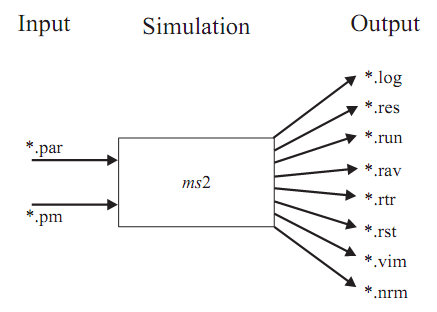
\includegraphics[width=0.55\columnwidth]{fig_structure.png}
	\caption{File structure needed and generated by \textit{ms}2.}
	\label{fig:File-structure}
\end{figure}




%
%
%\section{Running \textit{ms}2 on Windows or Linux}
%\label{sec:Running ms2 on Windows or Linux}
%% Simon
%
%\textbf{Restart a Simulation with \texttt{*.rst} file}
%


%
%\section{Running \textit{ms}2 in serial or parallel mode}
%\label{sec:Running ms2 in serial or parallel mode}
%% Simon


%
%
%\section{Flowchart}
%\label{sec:Flowchart}
%%Simon
%



\section{Input structure}
\label{sec:Input structure}
%Simon

\textit{ms}2 expects two input files: the \texttt{$^{*}$\hspace{-3pt}.par} and the \texttt{$^{*}$\hspace{-3pt}.pm} file. The \texttt{$^{*}$\hspace{-3pt}.par} file specifies the simulation \underline{par}ameters and the \texttt{.pm} file the molecular \underline{p}otential \underline{m}odel. The \texttt{$^{*}$\hspace{-3pt}.par} file is the main file steering the actual simulation. It contains all input variables for the simulation process, such as simulation type, ensemble, number of equilibration and production steps, time step length etc. Also the potential models need to be declared here. Each \texttt{$^{*}$\hspace{-3pt}.pm} file specifies exactly one chemical substance. To calculate mixtures, several \texttt{$^{*}$\hspace{-3pt}.pm} files have to be specified in the \texttt{$^{*}$\hspace{-3pt}.par} file.

Each line in both input file types sets one parameter, is empty or contains a comment. The comment symbol $\#$ and everything after it up to the end of the line is ignored by \textit{ms}2 in the same way as empty lines are. It is suggested to use only blanks instead of tabs, since the latter may cause trouble using input files generated on other platforms. 

A line setting a parameter in either \texttt{$^{*}$\hspace{-3pt}.par} or \texttt{$^{*}$\hspace{-3pt}.pm} file always consists of a keyword \texttt{XXX}, the \texttt{=} symbol and the parameter value YYY, e.\,g. \\
\texttt{NVTSteps  =  100000}\\
Leading spaces, trailing spaces and spaces surrounding = symbol are ignored. Parameter values can be strings in some case or numeric values. Parameter names and values that \textit{ms}2 expects for the parameter file and potential model files are described in sections \ref{sec:Keywords}. All parameters must be present in the input files in the certain order. The program reads the input file sequentially. % stimmt das noch? -> Martin B. fragen
Unidentified parameters are ignored. Missing or misplaced parameters lead to the termination of the program with the corresponding error message.


\subsection{Parameter file}
\label{sec:par - file}
% Simon

Below is an exemplary  \texttt{$^{*}$\hspace{-3pt}.par} file for a MD simulation of pure oxygen in the $NVT$ ensemble.  \texttt{$^{*}$\hspace{-3pt}.par} files are organised in three sections: the first section sets the general simulation parameters, such as timestep, MD or MC, unit systems etc. (lines 3 to 20 in the oxygen example), the second section sets the thermodynamic quantities to define the ensemble, such as temperature, density, number of components etc. (lines 21 to 26). The third section contains the potential models that shall be simulated and indicate their mole fraction (lines 28 to 31). The value for the keyword \texttt{PotModel} needs to be set according to the name of the potential model file that shall be used, including the tailing \texttt{$^{*}$\hspace{-3pt}.pm}. Each \texttt{$^{*}$\hspace{-3pt}.par} file ends with the cutoff that shall be applied throughout the simulation.\\
This example runs a MD simulation of pure oxygen at a constant temperature of 40\,K with an equilibration of 100.000 timesteps and a production period of 1.000.000 timesteps. The simulation contains 1372 molecules and uses a cutoff distance of 15\,\AA.

\vspace{0.7cm}
\begin{Verbatim}[frame=single,framesep=6.5mm,label=\fbox{*.par file for O$_2$ simulation},numbers=left,numbersep=-10pt,xrightmargin=5cm]
# ms2 parameter file 

Units         =       SI
LengthUnit    =       1.0
EnergyUnit    =     100.0
MassUnit      =      10.0
Simulation    =       MD
Integrator    =       Gear
TimeStep      =       0.001
Ensemble      =       NVT
MCORSteps     =       0
NVTSteps      =  100000
RunSteps      = 1000000
ResultFreq    =    1000
ErrorsFreq    =    5000
VisualFreq    =       0
CutoffMode    =       COM
LongRange     =       ReactionField
NEnsembles    =       1

# Ensemble 1
Temperature   =      60.0
Density       =      40.664
NParticles    =    1372
NComponents   =       1

# substances
PotModel      =       O2.pm
MoleFract     =       1.0
ChemPotMethod =       none

Cutoff        =      15.00
\end{Verbatim}
%Epsilon       =       1.0E10
\vspace{0.7cm}

Table~\ref{tab_KeywordsParFile} lists all input parameters and options to be specified in the \texttt{$^{*}$\hspace{-3pt}.par} file in section \ref{sec:Keywords}. The implemented methods behind these keywords are documented in section \ref{sec:Methods}. Creating a \texttt{$^{*}$\hspace{-3pt}.par} file is facilitated by the \textit{ms}2 feature program \textit{ms2}\textit{par}. Its use is described in detail in section \ref{sec:ms2par}.

% auf was muss verwiesen werden:
%- multiensemble 
%- res2gepar
%- 


\subsection{Potential model file}
\label{sec:pm - file}
% Simon

A \texttt{$^{*}$\hspace{-3pt}.pm} file contains the molecular model, also called force field, for a given substance. It contains the relative positions and parameters of all interaction sites. The potential model file for methanol is shown below. Methanol was modeled by two LJ sites and three point charges \parencite{Schnabel2007_A}. 

All positions and distances in the \texttt{$^{*}$\hspace{-3pt}.pm} file are given in \AA, the Lennard-Jones interaction parameters $\sigma$ and $\epsilon / k_{\text{B}}$ are given in \AA~and K, respectively, while the mass is given in atomic units (u$ = 1.6605\,\times 10^{-27}$ kg). The magnitudes of the charges are specified in electronic charges (e$ = 1.602 \times 10^{-19}$ C), while dipole moments and quadrupole moments are given in Debye ($\text{D} = 3.33564 \times 10^{-30}$ Cm) and Buckingham ($\text{B} = 3.33564 \times 10^{-40} \text{Cm}^{2}$), respectively. The orientations of the dipole and quadrupole are represented by spherical coordinates, where the azimuthal angle $\phi$ specifies the angle to the positive $x$ axis and the polar angle $\theta$ defines the angle to the positive $z$ axis. Both angles are specified in degrees. Molecular models can be orientated arbitrarily in the \texttt{$^{*}$\hspace{-3pt}.pm} file. All site positions are automatically transformed into a principal axes coordinate system at the beginning of each simulation run by \textit{ms}2. The normalized site positions are written to a \texttt{$^{*}$\hspace{-3pt}.nrm} output file for each component.


\vspace{0.7cm}
\begin{Verbatim}[frame=single,framesep=6.5mm,label=\fbox{*.pm file for methanol},numbers=left,numbersep=-10pt,xrightmargin=5cm]
# ms2 potential model file 

NSiteTypes  =  2

SiteType    =  LJ126
NSites      =  2

# CH3
x           =  7.660331e-01
y           =  1.338147e-02
z           =  0.0
sigma       =  3.7543
epsilon     =  120.592
mass        =  15.035

# O
x           =  -6.564695e-01
y           =  -6.389332e-02
z           =  0.0
sigma       =  3.030
epsilon     =  87.879
mass        =  15.999

SiteType    =  Charge
NSites      =  3

# H[e(1)]
x           =  -1.004989e+00
y           =  8.145993e-01
z           =  0.0
charge      =  +0.43128
mass        =  1.008

# e(2)
x           =  -6.564695e-01
y           =  -6.389332e-02
z           =  0.0
charge      =  -0.67874
mass        =  0.0

# e(1)
x           =  7.660331e-01
y           =  1.338147e-02
z           =  0.0
charge      =  +0.24746
mass        =  0.0

NRotAxes   =  auto
\end{Verbatim}
\vspace{0.7cm}


All input parameters and options to be specified in the \texttt{$^{*}$\hspace{-3pt}.pm} file are given in table \ref{tab:pmFile_keywords}. A \texttt{$^{*}$\hspace{-3pt}.pm} file has a specific structure, which is described in the following. The parameter \texttt{NSiteTypes} gives the number of different potential types (not the number of sites). Different potential types are 12-6 Lennard-Jones sites, point charges, point dipoles and point quadrupoles. Then the descriptions for each potential type follow sequentially. Each of them contains the number of sites of corresponding type \texttt{NSites}, followed by the definition of each individual site. Each site requires $x$, $y$ and $z$ coordinates and the mass in addition to its interaction parameters, depending on the site type. Lennard-Jones sites require one size and one energy parameter, point charges only the magnitude of the charge, while point dipoles and point quadrupoles require magnitude and orientation. At the end of a \texttt{$^{*}$\hspace{-3pt}.pm} file, the parameter \texttt{NRotAxes} is specified. Parameters \texttt{InertMomX}, \texttt{InertMomY} and \texttt{InertMomZ} are read if the moments of inertia are to be specified manually, set according to the \texttt{NRotAxes} value.



\renewcommand{\arraystretch}{1.2}
\begin{landscape}
	
	\small
	\setlength\tabcolsep{8pt}
	\begin{longtable}{llll}%[htbp]
		\toprule
		\onehalfspacing \textbf{keyword} & \textbf{value} & \textbf{explanation} & \textbf{recommended value} \\
		\bottomrule
		\endhead
		\midrule
		\multicolumn{4}{r}{\textit{Continued on next page}}
		\endfoot
		\bottomrule
		\caption{Parameters and options specified in a \texttt{$^{*}$\hspace{-3pt}.pm} file.} \\
		\endlastfoot
		&&&\\
%		\multicolumn{4}{l}{\textbf{Simulation specific}}\\
%		\midrule
	 \texttt{NSiteTypes} & \textit{int} & number of site types to appear in \texttt{$^{*}$\hspace{-3pt}.pm} file &  \\
	 \hline
	\texttt{SiteType} & \texttt{LJ126} & type of interaction site & must be specified \\
	& \texttt{Charge} & & \\
	& \texttt{Dipole} & & \\
	& \texttt{Quadrupole} & & \\
	\hline
	\texttt{NSites} & \textit{int} & number of sites for the corresponding interaction site type &  must be specified \\
	\hline
	\texttt{x} & \textit{double} & spatial coordinate of a site in \AA & must be specified for each site \\
	\texttt{y} & \textit{double} & spatial coordinate of a site in \AA & must be specified for each site \\
	\texttt{z} & \textit{double} & spatial coordinate of a site in \AA & must be specified for each site \\
	\hline
	\texttt{theta} & \textit{double} & angle $\theta$ between the dipole or quadrupole and the positive $z$ axis in degree & must be specified for dipole or quadrupole site\\                      
	\texttt{phi} & \textit{double} & angle $\phi$ between the dipole or quadrupole and the positive $x$ axis in degree & must be specified for dipole or quadrupole site\\
	\hline
	\texttt{sigma} & \textit{double} & Lennard-Jones radius $\sigma$ in \AA & must be specified for Lennard-Jones site \\
	\texttt{epsilon} & \textit{double} & Lennard-Jones energy $\varepsilon/k_{\text{B}}$ in K & must be specified for Lennard-Jones site\\
	\hline
	\texttt{charge} & \textit{double} & magnitude of point charge site & must be specified for charge site \\
	\texttt{dipole} & \textit{double} & dipole moment for dipole site & must be specified for dipolar site \\
	\texttt{quadrupole} & \textit{double} & quadrupole moment for quadrupole site & must be specified for quadrupolar site \\
	\hline
	\texttt{mass} & \textit{double} & mass in atomic units & must be specified for each site \\
	\hline
	\texttt{shielding} &\textit{double} & shielding radius in \AA~for MC steps & can be specified to get better convergence in MC run\\
	\hline
	\texttt{NRotAxes} & \texttt{auto} & number of rotation axes of the molecule & \texttt{auto}\\
	& \texttt{0} & & \\
	& \texttt{2} & & \\
	& \texttt{3}& & \\
	\hline
	\texttt{TotalMass} &\textit{double} & mass of molecule in atomic units & optional \\
	\hline
	\texttt{InertMomX} &\textit{double}& component of inertia moment in atomic mass unit multiplied by \AA$^{2}$ & if \texttt{NRotAxes} is 2 or 3\\
	\texttt{InertMomY} &\textit{double} & component of inertia moment in atomic mass unit multiplied by \AA$^{2}$ & if \texttt{NRotAxes} is 2 or 3\\
	\texttt{InertMomZ} &\textit{double} & component of inertia moment in atomic mass unit multiplied by \AA$^{2}$ & if \texttt{NRotAxes} is 3\\

		\label{tab:pmFile_keywords}
	\end{longtable}
\end{landscape}
\renewcommand{\arraystretch}{1}






%\section{Initial Conditions}
%\label{sec:Initial Conditions}
%% Simon


\section{Output structure}
\label{sec:Output structure}
% Simon

% Aufteilung in Standard und Optional (rtr, vim, rdf, thi) 

% Name of output files: by default the string of the input files * ending. Name can be manually ajusted.

% Tatjana:
%Restart geht jetzt mit "-r", also
%
%*/ms2  -r  ***.par
%
%Bei früheren Versionen konnte man mit dem rst file starten, geht jetzt aber glaube ich nicht mehr.
%*/ms2   ***.rst
%
%Wie lange noch gerechnet werden soll, legt entweder die Schrittzahl fest, oder du kannst auch die Walltime im par file festlegen.

% Simon:
%die Abwärtskompalitibiltät scheint nicht zu funktionieren?! die rst Veriante funktioniert nicht mehr.. -> ev. als Fußnote?!

\textit{ms}2 yields different output files depending on the specifications made in the \texttt{$^{*}$\hspace{-3pt}.par} file:
\begin{itemize}
	\item \texttt{$^{*}$\hspace{-3pt}.log} file - stores a complete summary of all execution steps taken by \textit{ms}2.
	\item \texttt{$^{*}$\hspace{-3pt}.res} file - contains the results of the simulation in an aggregated form. The data are written to file in reduced quantities as well as in SI units, along with the statistical uncertainties of the calculated properties. The *.res file is created during simulation and updated every specified number of time steps or loops. 
	\item \texttt{$^{*}$\hspace{-3pt}.run} file - contains the calculated properties of the simulation for a specified time step or loop interval. The file is in tabular form, where the data are given in reduced units. The file is subsequently updated according to the user specification, which is set in the *.par file.
	\item \texttt{$^{*}$\hspace{-3pt}.rav} file - contains the block averages of the calculated properties. The file is in tabular form, where the data are given in reduced units. The file is updated according to the user specification, which is set in the *.par file. 
	\item \texttt{$^{*}$\hspace{-3pt}.rst} file - is the restart file of the simulation. It contains all molecular positions, velocities, orientations, forces, torques and block averages for the thermodynamic properties. It is written once at the end of a simulation or immediately after having received a termination signal of the operating system. The *.rst file allows for a stepwise execution of the simulation, necessary e.g. in case of an early interruption of the simulation, time limits on a queuing system or unexpected halts.
	\item \texttt{$^{*}$\hspace{-3pt}.vim} file - is the trajectory visualization file. It contains the positions and orientations of all molecules in an aggregated ASCII format. The configurations are written to file after a user-specified interval of time steps or loops. The *.vim file is readable by the visualization tool \textit{ms}2\textit{molecules}, which is also part of the simulation package.
	\item \texttt{$^{*}$\hspace{-3pt}.nrm} file - stores the normalized coordinates of a potential model after a principal axes transformation.
	\item \texttt{$^{*}$\hspace{-3pt}.rtr} file - stores the final value of the autocorrelation functions and their integrals. The number of output lines is equal to Corrlength divided by StepsCorrfun. The number of output lines has to be defined in the *.par file.
%	\item \texttt{$^{*}$\hspace{-3pt}.rdf} file - 
%	\item \texttt{$^{*}$\hspace{-3pt}.thi} file - 
\end{itemize}

%The next section provides some output files to illustrate the structure of them.

%\subsection{log - file}
%\label{sec:log - file}
%
%
%
%\subsection{res - file}
%\label{sec:res - file}
%
%
%\subsection{rav - file}
%\label{sec:rav - file}
%
%
%
%\subsection{rst - file}
%\label{sec:rst - file}
%
%
%
%\subsection{vim - file}
%\label{sec:vim - file}
%
%
%
%\subsection{nrm - file}
%\label{sec:nrm - file}
%
%
%
%\subsection{rdf - file}
%\label{sec:rdf - file}
%
%
%\subsection{thi - file}
%\label{sec:thi -file}




%\section{Command line options}
%\label{sec:Command line options}
% Simon

% in ms2_global ab Zeile 1131

% give name for Output Data, different from default: put string behind the *par file in the command line to run a job. 
